% defer/rcufundamental.tex

\subsection{RCU Fundamentals}
\label{sec:defer:RCU Fundamentals}

Authors: Paul E. McKenney and Jonathan Walpole

Read-copy update (RCU) is a synchronization mechanism that was added to
the Linux kernel in October of 2002.
RCU achieves scalability
improvements by allowing reads to occur concurrently with updates.
In contrast with conventional locking primitives that ensure mutual exclusion
among concurrent threads regardless of whether they be readers or
updaters, or with reader-writer locks that allow concurrent reads but not in
the presence of updates, RCU supports concurrency between a single
updater and multiple readers.
RCU ensures that reads are coherent by
maintaining multiple versions of objects and ensuring that they are not
freed up until all pre-existing read-side critical sections complete.
RCU defines and uses efficient and scalable mechanisms for publishing
and reading new versions of an object, and also for deferring the collection
of old versions.
These mechanisms distribute the work among read and
update paths in such a way as to make read paths extremely fast. In some
cases (non-preemptable kernels), RCU's read-side primitives have zero
overhead.

\QuickQuiz{But doesn't seqlock also permit readers and updaters to get
work done concurrently?}
\QuickQuizAnswer{
Yes and no.
Although seqlock readers can run concurrently with
seqlock writers, whenever this happens, the {\tt read\_seqretry()}
primitive will force the reader to retry.
This means that any work done by a seqlock reader running concurrently
with a seqlock updater will be discarded and redone.
So seqlock readers can \emph{run} concurrently with updaters,
but they cannot actually get any work done in this case.

In contrast, RCU readers can perform useful work even in presence
of concurrent RCU updaters.
} \QuickQuizEnd

This leads to the question ``what exactly is RCU?'', and perhaps also
to the question ``how can RCU \emph{possibly} work?'' (or, not
infrequently, the assertion that RCU cannot possibly work).
This document addresses these questions from a fundamental viewpoint;
later installments look at them from usage and from API viewpoints.
This last installment also includes a list of references.

RCU is made up of three fundamental mechanisms, the first being
used for insertion, the second being used for deletion, and the third
being used to allow readers to tolerate concurrent insertions and deletions.
Section~\ref{sec:defer:Publish-Subscribe Mechanism}
describes the publish-subscribe mechanism used for insertion,
Section~\ref{sec:defer:Wait For Pre-Existing RCU Readers to Complete}
describes how waiting for pre-existing RCU readers enabled deletion,
and
Section~\ref{sec:defer:Maintain Multiple Versions of Recently Updated Objects}
discusses how maintaining multiple versions of recently updated objects
permits concurrent insertions and deletions.
Finally,
Section~\ref{sec:defer:Summary of RCU Fundamentals}
summarizes RCU fundamentals.

\subsubsection{Publish-Subscribe Mechanism}
\label{sec:defer:Publish-Subscribe Mechanism}

\begin{figure}[tbp]
{ \scriptsize
\begin{verbatim}
  1 struct foo {
  2   int a;
  3   int b;
  4   int c;
  5 };
  6 struct foo *gp = NULL;
  7 
  8 /* . . . */
  9 
 10 p = kmalloc(sizeof(*p), GFP_KERNEL);
 11 p->a = 1;
 12 p->b = 2;
 13 p->c = 3;
 14 gp = p;
\end{verbatim}
}
\caption{Data Structure Publication (Unsafe)}
\label{fig:defer:Data Structure Publication (Unsafe)}
\end{figure}

One key attribute of RCU is the ability to safely scan data, even
though that data is being modified concurrently.
To provide this ability for concurrent insertion,
RCU uses what can be thought of as a publish-subscribe mechanism.
For example, consider an initially \url{NULL} global pointer
\url{gp} that is to be modified to point to a newly allocated
and initialized data structure.
The code fragment shown in
Figure~\ref{fig:defer:Data Structure Publication (Unsafe)}
(with the addition of appropriate locking)
might be used for this purpose.

Unfortunately, there is nothing forcing the compiler and CPU to execute
the last four assignment statements in order.
If the assignment to \url{gp} happens before the initialization
of \url{p} fields, then concurrent readers could see the
uninitialized values.
Memory barriers are required to keep things ordered, but memory barriers
are notoriously difficult to use.
We therefore encapsulate them into a primitive
\url{rcu_assign_pointer()} that has publication semantics.
The last four lines would then be as follows:

\vspace{5pt}
\begin{minipage}[t]{\columnwidth}
\begin{verbatim}
  1 p->a = 1;
  2 p->b = 2;
  3 p->c = 3;
  4 rcu_assign_pointer(gp, p);
\end{verbatim}
\end{minipage}
\vspace{5pt}

The \url{rcu_assign_pointer()}
would \emph{publish} the new structure, forcing both the compiler
and the CPU to execute the assignment to \url{gp} \emph{after}
the assignments to the fields referenced by \url{p}

However, it is not sufficient to only enforce ordering at the
updater, as the reader must enforce proper ordering as well.
Consider for example the following code fragment:

\vspace{5pt}
\begin{minipage}[t]{\columnwidth}
\begin{verbatim}
  1 p = gp;
  2 if (p != NULL) {
  3   do_something_with(p->a, p->b, p->c);
  4 }
\end{verbatim}
\end{minipage}
\vspace{5pt}

Although this code fragment might well seem immune to misordering,
unfortunately, the
DEC Alpha CPU~\cite{PaulMcKenney2005i,PaulMcKenney2005j}
and value-speculation compiler optimizations can, believe it or not,
cause the values of \url{p->a}, \url{p->b}, and
\url{p->c} to be fetched before the value of \url{p}.
This is perhaps easiest to see in the case of value-speculation
compiler optimizations, where the compiler guesses the value
of \url{p} fetches \url{p->a}, \url{p->b}, and
\url{p->c} then fetches the actual value of \url{p}
in order to check whether its guess was correct.
This sort of optimization is quite aggressive, perhaps insanely so,
but does actually occur in the context of profile-driven optimization.

Clearly, we need to prevent this sort of skullduggery on the
part of both the compiler and the CPU.
The \url{rcu_dereference()} primitive uses
whatever memory-barrier instructions and compiler
directives are required for this purpose:

\vspace{5pt}
\begin{minipage}[t]{\columnwidth}
\begin{verbatim}
  1 rcu_read_lock();
  2 p = rcu_dereference(gp);
  3 if (p != NULL) {
  4   do_something_with(p->a, p->b, p->c);
  5 }
  6 rcu_read_unlock();
\end{verbatim}
\end{minipage}
\vspace{5pt}

The \url{rcu_dereference()} primitive can thus be thought of
as \emph{subscribing} to a given value of the specified pointer,
guaranteeing that subsequent dereference operations will see any
initialization that occurred before the corresponding publish
(\url{rcu_assign_pointer()} operation.
The \url{rcu_read_lock()} and \url{rcu_read_unlock()}
calls are absolutely required: they define the extent of the
RCU read-side critical section.
Their purpose is explained in
Section~\ref{sec:defer:Wait For Pre-Existing RCU Readers to Complete},
however, they never spin or block, nor do they prevent the
\url{list_add_rcu()} from executing concurrently.
In fact, in non-\url{CONFIG_PREEMPT} kernels, they generate
absolutely no code.  

\begin{figure}[tb]
\begin{center}
\resizebox{3in}{!}{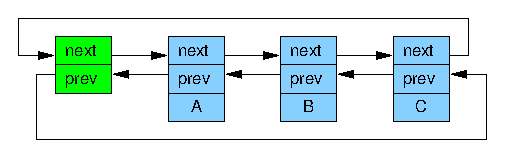
\includegraphics{defer/Linux_list}}
\end{center}
\caption{Linux Circular Linked List}
\label{fig:defer:Linux Circular Linked List}
\end{figure}

\begin{figure}[tb]
\begin{center}
\resizebox{3in}{!}{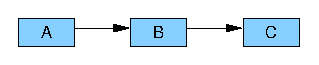
\includegraphics{defer/Linux_list_abbr}}
\end{center}
\caption{Linux Linked List Abbreviated}
\label{fig:defer:Linux Linked List Abbreviated}
\end{figure}

Although \url{rcu_assign_pointer()} and
\url{rcu_dereference()} can in theory be used to construct any
conceivable RCU-protected data structure, in practice it is often better
to use higher-level constructs.
Therefore, the \url{rcu_assign_pointer()} and
\url{rcu_dereference()}
primitives have been embedded in special RCU variants of Linux's
list-manipulation API.
Linux has two variants of doubly linked list, the circular
{\tt struct list\_head} and the linear
{\tt struct hlist\_head}/{\tt struct hlist\_node} pair.
The former is laid out as shown in
Figure~\ref{fig:defer:Linux Circular Linked List},
where the green boxes represent
the list header and the blue boxes represent the elements in the
list.
This notation is cumbersome, and will therefore be abbreviated as shown in 
Figure~\ref{fig:defer:Linux Linked List Abbreviated}.

\begin{figure}[tbp]
{ \scriptsize
\begin{verbatim}
  1 struct foo {
  2   struct list_head *list;
  3   int a;
  4   int b;
  5   int c;
  6 };
  7 LIST_HEAD(head);
  8 
  9 /* . . . */
 10 
 11 p = kmalloc(sizeof(*p), GFP_KERNEL);
 12 p->a = 1;
 13 p->b = 2;
 14 p->c = 3;
 15 list_add_rcu(&p->list, &head);
\end{verbatim}
}
\caption{RCU Data Structure Publication}
\label{fig:defer:RCU Data Structure Publication}
\end{figure}

Adapting the pointer-publish example for the linked list results in
the code shown in
Figure~\ref{fig:defer:RCU Data Structure Publication}.

Line~15 must be protected by some synchronization mechanism (most
commonly some sort of lock) to prevent multiple \url{list_add()}
instances from executing concurrently.
However, such synchronization does not prevent this \url{list_add()}
instance from executing concurrently with RCU readers.

Subscribing to an RCU-protected list is straightforward:

\vspace{5pt}
\begin{minipage}[t]{\columnwidth}
\scriptsize
\begin{verbatim}
  1 rcu_read_lock();
  2 list_for_each_entry_rcu(p, head, list) {
  3   do_something_with(p->a, p->b, p->c);
  4 }
  5 rcu_read_unlock();
\end{verbatim}
\end{minipage}
\vspace{5pt}

The \url{list_add_rcu()} primitive publishes
an entry into the specified list, guaranteeing that the corresponding
\url{list_for_each_entry_rcu()} invocation will properly
subscribe to this same entry.

\QuickQuiz{What prevents the {\tt list\_for\_each\_entry\_rcu()} from
getting a segfault if it happens to execute at exactly the same
time as the {\tt list\_add\_rcu()}?}
\QuickQuizAnswer{
On all systems running Linux, loads from and stores
to pointers are atomic, that is, if a store to a pointer occurs at
the same time as a load from that same pointer, the load will return
either the initial value or the value stored, never some bitwise mashup
of the two.
In addition, the {\tt list\_for\_each\_entry\_rcu()} always proceeds
forward through the list, never looking back.
Therefore, the {\tt list\_for\_each\_entry\_rcu()} will either see
the element being added by {\tt list\_add\_rcu()} or it will not,
but either way, it will see a valid well-formed list.
} \QuickQuizEnd

\begin{figure}[tb]
\begin{center}
\resizebox{3in}{!}{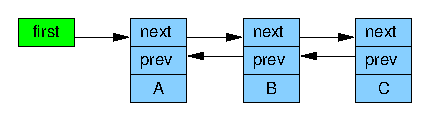
\includegraphics{defer/Linux_hlist}}
\end{center}
\caption{Linux Linear Linked List}
\label{fig:defer:Linux Linear Linked List}
\end{figure}

Linux's other doubly linked list, the hlist,
is a linear list, which means that
it needs only one pointer for the header rather than the two
required for the circular list, as shown in
Figure\ref{fig:defer:Linux Linear Linked List}.
Thus, use of hlist can halve the memory consumption for the hash-bucket
arrays of large hash tables.
As before, this notation is cumbersome, so hlists will be abbreviated
in the same way lists are, as shown in
Figure~\ref{fig:defer:Linux Linked List Abbreviated}.

\begin{figure}[tbp]
{ \scriptsize
\begin{verbatim}
  1 struct foo {
  2   struct hlist_node *list;
  3   int a;
  4   int b;
  5   int c;
  6 };
  7 HLIST_HEAD(head);
  8 
  9 /* . . . */
 10 
 11 p = kmalloc(sizeof(*p), GFP_KERNEL);
 12 p->a = 1;
 13 p->b = 2;
 14 p->c = 3;
 15 hlist_add_head_rcu(&p->list, &head);
\end{verbatim}
}
\caption{RCU {\tt hlist} Publication}
\label{fig:defer:RCU hlist Publication}
\end{figure}

Publishing a new element to an RCU-protected hlist is quite similar
to doing so for the circular list,
as shown in Figure~\ref{fig:defer:RCU hlist Publication}.

As before, line~15 must be protected by some sort of synchronization
mechanism, for example, a lock.

Subscribing to an RCU-protected hlist is also similar to the
circular list:

\vspace{5pt}
\begin{minipage}[t]{\columnwidth}
\scriptsize
\begin{verbatim}
  1 rcu_read_lock();
  2 hlist_for_each_entry_rcu(p, q, head, list) {
  3   do_something_with(p->a, p->b, p->c);
  4 }
  5 rcu_read_unlock();
\end{verbatim}
\end{minipage}
\vspace{5pt}

\QuickQuiz{Why do we need to pass two pointers into
{\tt hlist\_for\_each\_entry\_rcu()}
when only one is needed for {\tt list\_for\_each\_entry\_rcu()}?}
\QuickQuizAnswer{
Because in an hlist it is necessary to check for
NULL rather than for encountering the head.
(Try coding up a single-pointer {\tt hlist\_for\_each\_entry\_rcu()}
If you come up with a nice solution, it would be a very good thing!)
} \QuickQuizEnd

\begin{table*}[tb]
\begin{center}
\scriptsize
\begin{tabular}{l||l|l|l}
Category  & Publish	& Retract	& Subscribe \\
\hline
\hline
Pointers  & \url{rcu_assign_pointer()}
			& \url{rcu_assign_pointer(..., NULL)}
					& \url{rcu_dereference()} \\
\hline
Lists     & \parbox{1.5in}{
		\url{list_add_rcu()} \\
		\url{list_add_tail_rcu()} \\
		\url{list_replace_rcu()} }
			& \url{list_del_rcu()}
					& \url{list_for_each_entry_rcu()} \\
\hline
Hlists    & \parbox{1.5in}{
		\url{hlist_add_after_rcu()} \\
		\url{hlist_add_before_rcu()}  \\
		\url{hlist_add_head_rcu()} \\
		\url{hlist_replace_rcu()} }
			& \url{hlist_del_rcu()}
					& \url{hlist_for_each_entry_rcu()}
\end{tabular}
\end{center}
\caption{RCU Publish and Subscribe Primitives}
\label{tab:defer:RCU Publish and Subscribe Primitives}
\end{table*}

The set of RCU publish and subscribe primitives are shown in
Table~\ref{tab:defer:RCU Publish and Subscribe Primitives},
along with additional primitives to ``unpublish'', or retract.

Note that the \url{list_replace_rcu()}, \url{list_del_rcu()},
\url{hlist_replace_rcu()}, and \url{hlist_del_rcu()}
APIs add a complication.
When is it safe to free up the data element that was replaced or
removed?
In particular, how can we possibly know when all the readers
have released their references to that data element?

These questions are addressed in the following section.

\subsubsection{Wait For Pre-Existing RCU Readers to Complete}
\label{sec:defer:Wait For Pre-Existing RCU Readers to Complete}

In its most basic form, RCU is a way of waiting for things to finish.
Of course, there are a great many other ways of waiting for things to
finish, including reference counts, reader-writer locks, events, and so on.
The great advantage of RCU is that it can wait for each of
(say) 20,000 different things without having to explicitly
track each and every one of them, and without having to worry about
the performance degradation, scalability limitations, complex deadlock
scenarios, and memory-leak hazards that are inherent in schemes
using explicit tracking.

In RCU's case, the things waited on are called
``RCU read-side critical sections''.
An RCU read-side critical section starts with an
\url{rcu_read_lock()} primitive, and ends with a corresponding
\url{rcu_read_unlock()} primitive.
RCU read-side critical sections can be nested, and may contain pretty
much any code, as long as that code does not explicitly block or sleep
(although a special form of RCU called SRCU~\cite{PaulEMcKenney2006c}
does permit general sleeping in SRCU read-side critical sections).
If you abide by these conventions, you can use RCU to wait for \emph{any}
desired piece of code to complete.

RCU accomplishes this feat by indirectly determining when these
other things have finished~\cite{PaulEMcKenney2007whatisRCU,
PaulEMcKenney2007PreemptibleRCU}.  \emph{@@@ add reference to implementation
sections @@@}

\begin{figure}[tb]
\begin{center}
\resizebox{3in}{!}{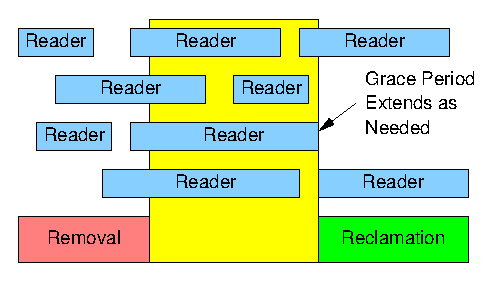
\includegraphics{defer/GracePeriodGood}}
\end{center}
\caption{Readers and RCU Grace Period}
\label{fig:defer:Readers and RCU Grace Period}
\end{figure}

In particular, as shown in
Figure~\ref{fig:defer:Readers and RCU Grace Period},
RCU is a way of
waiting for pre-existing RCU read-side critical sections to completely
finish, including memory operations executed by those critical sections.
However, note that RCU read-side critical sections
that begin after the beginning
of a given grace period can and will extend beyond the end of that grace
period.

The following pseudocode shows the basic form of algorithms that use
RCU to wait for readers:

\begin{enumerate}
\item	Make a change, for example, replace an element in a linked list.
\item	Wait for all pre-existing RCU read-side critical sections to
	completely finish (for example, by using the
	\url{synchronize_rcu()} primitive).
	The key observation here is that subsequent RCU read-side critical
	sections have no way to gain a reference to the newly removed
	element.
\item	Clean up, for example, free the element that was replaced above.
\end{enumerate}

\begin{figure}[tbp]
{ \scriptsize
\begin{verbatim}
  1 struct foo {
  2   struct list_head *list;
  3   int a;
  4   int b;
  5   int c;
  6 };
  7 LIST_HEAD(head);
  8 
  9 /* . . . */
 10 
 11 p = search(head, key);
 12 if (p == NULL) {
 13   /* Take appropriate action, unlock, and return. */
 14 }
 15 q = kmalloc(sizeof(*p), GFP_KERNEL);
 16 *q = *p;
 17 q->b = 2;
 18 q->c = 3;
 19 list_replace_rcu(&p->list, &q->list);
 20 synchronize_rcu();
 21 kfree(p);
\end{verbatim}
}
\caption{Canonical RCU Replacement Example}
\label{fig:defer:Canonical RCU Replacement Example}
\end{figure}

The code fragment shown in
Figure~\ref{fig:defer:Canonical RCU Replacement Example},
adapted from those in Section~\ref{sec:defer:Publish-Subscribe Mechanism},
demonstrates this process, with field \url{a} being the search key.

Lines~19, 20, and 21 implement the three steps called out above.
Lines~16-19 gives RCU (``read-copy update'') its name: while permitting
concurrent \emph{reads}, line~16 \emph{copies} and lines~17-19
do an \emph{update}.

The \url{synchronize_rcu()} primitive might seem a bit
mysterious at first.
After all, it must wait for all RCU read-side critical sections to
complete, and, as we saw earlier, the
\url{rcu_read_lock()} and \url{rcu_read_unlock()} primitives
that delimit RCU read-side critical sections don't even generate any
code in non-\url{CONFIG_PREEMPT} kernels!

There is a trick, and the trick is that RCU Classic read-side critical
sections delimited by \url{rcu_read_lock()} and
\url{rcu_read_unlock()} are not permitted to block or sleep.
Therefore, when a given CPU executes a context switch, we are guaranteed
that any prior RCU read-side critical sections will have completed.
This means that as soon as each
CPU has executed at least one context switch, \emph{all}
prior RCU read-side critical sections are guaranteed to have completed,
meaning that \url{synchronize_rcu()} can safely return.

Thus, RCU Classic's \url{synchronize_rcu()}
can conceptually be as simple as the following:

\vspace{5pt}
\begin{minipage}[t]{\columnwidth}
\begin{verbatim}
  1 for_each_online_cpu(cpu)
  2   run_on(cpu);
\end{verbatim}
\end{minipage}
\vspace{5pt}

Here, \url{run_on()} switches the current thread to the
specified CPU, which forces a context switch on that CPU.
The \url{for_each_online_cpu()} loop therefore forces a
context switch on each CPU, thereby guaranteeing that all prior
RCU read-side critical sections have completed, as required.
Although this simple approach works for kernels in which preemption
is disabled across RCU read-side critical sections, in other
words, for non-\url{CONFIG_PREEMPT} and \url{CONFIG_PREEMPT}
kernels, it does \emph{not} work for \url{CONFIG_PREEMPT_RT}
realtime (-rt) kernels.
Therefore, realtime RCU uses a different approach based loosely on reference
counters~\cite{PaulEMcKenney2007PreemptibleRCU}.

Of course, the actual implementation in the Linux kernel
is much more complex, as it is required
to handle interrupts, NMIs, CPU hotplug, and other hazards of
production-capable kernels, but while also maintaining good performance and
scalability.
Realtime implementations of RCU must additionally help provide good
realtime response, which rules out implementations (like the simple
two-liner above) that rely on disabling preemption.

Although it is good to know that there is a simple conceptual
implementation of \url{synchronize_rcu()}, other questions remain.
For example, what exactly do RCU
readers see when traversing a concurrently updated list?
This question is addressed in the following section.

\subsubsection{Maintain Multiple Versions of Recently Updated Objects}
\label{sec:defer:Maintain Multiple Versions of Recently Updated Objects}

This section demonstrates how RCU maintains multiple versions of
lists to accommodate synchronization-free readers.
Two examples are presented showing how an element
that might be referenced by a given reader must remain intact
while that reader remains in its RCU read-side critical section.
The first example demonstrates deletion of a list element,
and the second example demonstrates replacement of an element.

\paragraph{Example 1: Maintaining Multiple Versions During Deletion}
\label{sec:defer:Example 1: Maintaining Multiple Versions During Deletion}

To start the ``deletion'' example,
we will modify lines~11-21 in
Figure~\ref{fig:defer:Canonical RCU Replacement Example}
to read as follows:

\vspace{5pt}
\begin{minipage}[t]{\columnwidth}
\begin{verbatim}
  1 p = search(head, key);
  2 if (p != NULL) {
  3   list_del_rcu(&p->list);
  4   synchronize_rcu();
  5   kfree(p);
  6 }
\end{verbatim}
\end{minipage}
\vspace{5pt}

\begin{figure}[tb]
\begin{center}
\resizebox{3in}{!}{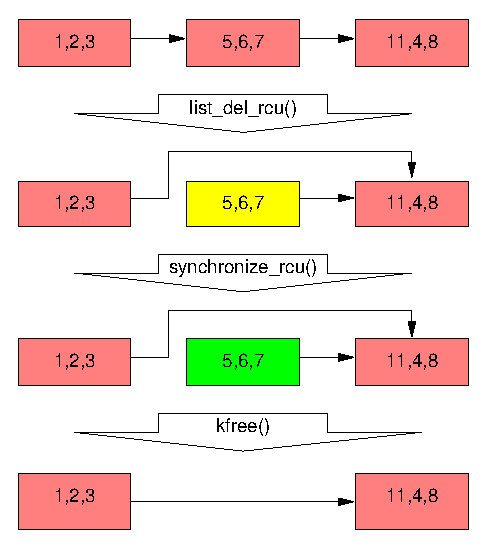
\includegraphics{defer/RCUDeletion}}
\end{center}
\caption{RCU Deletion From Linked List}
\label{fig:defer:RCU Deletion From Linked List}
\end{figure}

This code will update the list as shown in
Figure~\ref{fig:defer:RCU Deletion From Linked List}.
The triples in each element represent the values of fields \url{a},
\url{b}, and \url{c}, respectively.
The red-shaded elements
indicate that RCU readers might be holding references to them.
Please note that 
we have omitted the backwards pointers and the link from the tail
of the list to the head for clarity.

After the \url{list_del_rcu()} on
line~3 has completed, the \url{5,6,7}~element
has been removed from the list, as shown in the second row of
Figure~\ref{fig:defer:RCU Deletion From Linked List}.
Since readers do not synchronize directly with updaters,
readers might be concurrently scanning this list.
These concurrent readers might or might not see the newly removed element,
depending on timing.
However, readers that were delayed (e.g., due to interrupts, ECC memory
errors, or, in \url{CONFIG_PREEMPT_RT} kernels, preemption)
just after fetching a pointer to the newly removed element might
see the old version of the list for quite some time after the
removal.
Therefore, we now have two versions of the list, one with element
\url{5,6,7} and one without.
The \url{5,6,7}~element is
shaded yellow, indicating
that old readers might still be referencing it, but that new
readers cannot obtain a reference to it.

Please note that readers are not permitted to maintain references to
element~\url{5,6,7} after exiting from their RCU read-side
critical sections.
Therefore,
once the \url{synchronize_rcu()} on
line~4 completes, so that all pre-existing readers are
guaranteed to have completed,
there can be no more readers referencing this
element, as indicated by its green shading on the third row of
Figure~\ref{fig:defer:RCU Deletion From Linked List}.
We are thus back to a single version of the list.

At this point, the \url{5,6,7}~element may safely be
freed, as shown on the final row of
Figure~\ref{fig:defer:RCU Deletion From Linked List}.
At this point, we have completed the deletion of
element~\url{5,6,7}.
The following section covers replacement.

\paragraph{Example 2: Maintaining Multiple Versions During Replacement}
\label{sec:defer:Example 2: Maintaining Multiple Versions During Replacement}

To start the replacement example,
here are the last few lines of the
example shown in
Figure~\ref{fig:defer:Canonical RCU Replacement Example}:

\vspace{5pt}
\begin{minipage}[t]{\columnwidth}
\begin{verbatim}
  1 q = kmalloc(sizeof(*p), GFP_KERNEL);
  2 *q = *p;
  3 q->b = 2;
  4 q->c = 3;
  5 list_replace_rcu(&p->list, &q->list);
  6 synchronize_rcu();
  7 kfree(p);
\end{verbatim}
\end{minipage}
\vspace{5pt}

\begin{figure}[tbp]
\begin{center}
\resizebox{2.7in}{!}{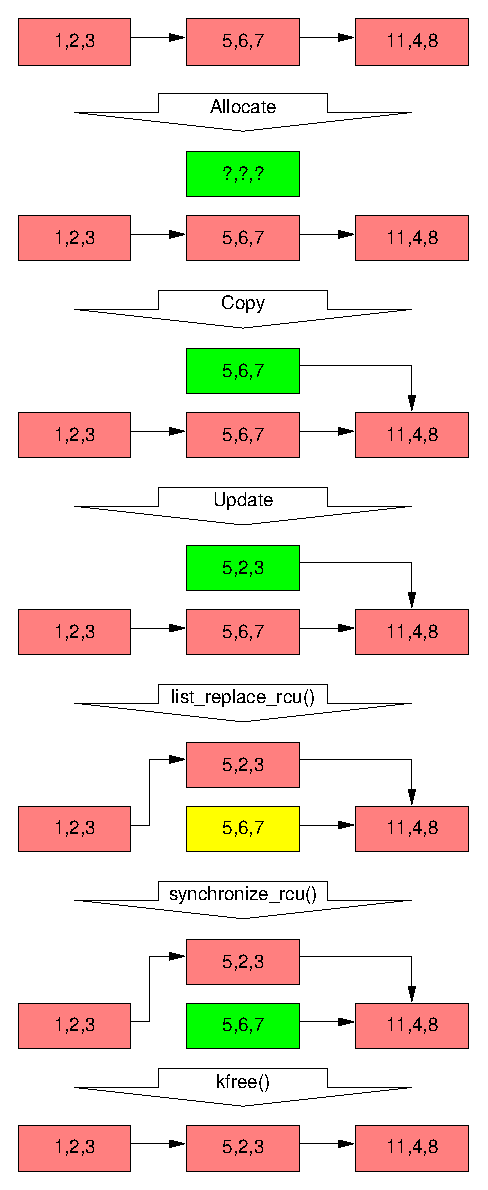
\includegraphics{defer/RCUReplacement}}
\end{center}
\caption{RCU Replacement in Linked List}
\label{fig:defer:RCU Replacement in Linked List}
\end{figure}

The initial state of the list, including the pointer \url{p},
is the same as for the deletion example, as shown on the
first row of
Figure~\ref{fig:defer:RCU Replacement in Linked List}.

As before,
the triples in each element represent the values of fields \url{a},
\url{b}, and \url{c}, respectively.
The red-shaded elements might be referenced by readers,
and because readers do not synchronize directly with updaters,
readers might run concurrently with this entire replacement process.
Please note that 
we again omit the backwards pointers and the link from the tail
of the list to the head for clarity.

Line~1 \url{kmalloc()}s a replacement element, as follows,
resulting in the state as shown in the second row of
Figure~\ref{fig:defer:RCU Replacement in Linked List}.
At this point, no reader can hold a reference to the newly allocated
element (as indicated by its green shading), and it is uninitialized
(as indicated by the question marks).

Line~2 copies the old element to the new one, resulting in the
state as shown in the third row of
Figure~\ref{fig:defer:RCU Replacement in Linked List}.
The newly allocated element still cannot be referenced by readers, but
it is now initialized.

Line~3 updates \url{q->b} to the value ``2'', and
line~4 updates \url{q->c} to the value ``3'', as shown on the fourth row of
Figure~\ref{fig:defer:RCU Replacement in Linked List}.

Now, line~5 does the replacement, so that the new element is
finally visible to readers, and hence is shaded red, as shown on
the fifth row of
Figure~\ref{fig:defer:RCU Replacement in Linked List}.
At this point, as shown below, we have two versions of the list.
Pre-existing readers might see the \url{5,6,7} element (which is
therefore now shaded yellow), but
new readers will instead see the \url{5,2,3} element.
But any given reader is guaranteed to see some well-defined list.

After the \url{synchronize_rcu()} on line~6 returns,
a grace period will have elapsed, and so all reads that started before the
\url{list_replace_rcu()} will have completed.
In particular, any readers that might have been holding references
to the \url{5,6,7} element are guaranteed to have exited
their RCU read-side critical sections, and are thus prohibited from
continuing to hold a reference.
Therefore, there can no longer be any readers holding references
to the old element, as indicated its green shading in the sixth row of
Figure~\ref{fig:defer:RCU Replacement in Linked List}.
As far as the readers are concerned, we are back to having a single version
of the list, but with the new element in place of the old.

After the \url{kfree()} on line 7 completes, the list will
appear as shown on the final row of
Figure~\ref{fig:defer:RCU Replacement in Linked List}.

Despite the fact that RCU was named after the replacement case,
the vast majority of RCU usage within the Linux kernel relies on
the simple deletion case shown in
Section~\ref{sec:defer:Maintain Multiple Versions of Recently Updated Objects}.

\paragraph{Discussion}
\label{sec:defer:Discussion}

These examples assumed that a mutex was held across the entire
update operation, which would mean that there could be at most two
versions of the list active at a given time.

\QuickQuiz{How would you modify the deletion example to permit more than two
versions of the list to be active?}
\QuickQuizAnswer{
One way of accomplishing this is as shown in
Figure~\ref{fig:defer:Concurrent RCU Deletion}.

\begin{figure}[htbp]
{ \centering
\begin{verbatim}
  1 spin_lock(&mylock);
  2 p = search(head, key);
  3 if (p == NULL)
  4   spin_unlock(&mylock);
  5 else {
  6   list_del_rcu(&p->list);
  7   spin_unlock(&mylock);
  8   synchronize_rcu();
  9   kfree(p);
 10 }
\end{verbatim}
}
\caption{Concurrent RCU Deletion}
\label{fig:defer:Concurrent RCU Deletion}
\end{figure}

Note that this means that multiple concurrent deletions might be
waiting in {\tt synchronize\_rcu()}.
} \QuickQuizEnd

\QuickQuiz{How many RCU versions of a given list can be
active at any given time?}
\QuickQuizAnswer{
That depends on the synchronization design.
If a semaphore protecting the update is held across the grace period,
then there can be at most two versions, the old and the new.

However, if only the search, the update, and the
{\tt list\_replace\_rcu()} were protected by a lock, then
there could be an arbitrary number of versions active, limited only
by memory and by how many updates could be completed within a
grace period.
But please note that data structures that are updated so frequently
probably are not good candidates for RCU.
That said, RCU can handle high update rates when necessary.
} \QuickQuizEnd

This sequence of events shows how RCU updates use multiple versions
to safely carry out changes in presence of concurrent readers.
Of course, some algorithms cannot gracefully handle multiple versions.
There are techniques
for adapting such algorithms to RCU~\cite{PaulEdwardMcKenneyPhD},
but these are beyond the scope of this section.

\subsubsection{Summary of RCU Fundamentals}
\label{sec:defer:Summary of RCU Fundamentals}

This section has described the three fundamental components of RCU-based
algorithms:

\begin{enumerate}
\item	a publish-subscribe mechanism for adding new data,

\item	a way of waiting for pre-existing RCU readers to finish, and

\item	a discipline of maintaining multiple versions to permit
	change without harming or unduly delaying concurrent RCU readers.
\end{enumerate}

\QuickQuiz{How can RCU updaters possibly delay RCU readers, given that the
{\tt rcu\_read\_lock()} and {\tt rcu\_read\_unlock()}
primitives neither spin nor block?}
\QuickQuizAnswer{
The modifications undertaken by a given RCU updater will cause the
corresponding CPU to invalidate cache lines containing the data,
forcing the CPUs running concurrent RCU readers to incur expensive
cache misses.
(Can you design an algorithm that changes a data structure \emph{without}
inflicting expensive cache misses on concurrent readers?
On subsequent readers?)
} \QuickQuizEnd

These three RCU components
allow data to be updated in face of concurrent readers, and
can be combined in different ways to
implement a surprising variety of different types of RCU-based algorithms,
some of which are described in the following section.

\emph{@@@ state-space reduction, perhaps in usage section @@@}
